The following literature review explores mesh networks in a wooded area,When communicating from two devices across a network there are many of issues associated with this communication such as signal loss due to:
	\begin{itemize}
		\item Environmental conditions such as rain .lighting etc
		\item Whether the device's antenna are in line of sight with each other
		\item If the devices are in the line of sight with each other. We can still reflections from a multi-path environment
		\item Possibility of falling trees obstructing the path of the signal causing more attenuation in the signal strength
	\end{itemize}
	In this project aims explore mesh networks and transmit data across them,  a mesh network is a type of network where no node in the network acts as a  master.A node is a device which has a transceiver.As we look at the environment in which this project will be carried out, we can expect different phenomena to occur such as  Attenuation According to ITU \cite{ITU} "Attenuation due to vegetation varies widely due to the irregular Nature of the medium and the wide range of species, densities and water content obtained in practice"
	Transmitting any radio wave takes energy ,Another factor to consider is whether wind will cause a  delay in the signal. This report aims to show my findings and try to account for environmental conditions
	\subsection{Overview} \label{sec: overview}

		The following section provides a brief overview of  this project on mesh networks in a forest the following question is:
		
		\begin{enumerate}
			\item What frequencies can transmit in a forest
			\begin{itemize}
				\item What are the disadvantages of transmitting at this range
				\item What are the effects of the multi-path environment when there is a line of sight
				\item What happens to bon-line of sight
			\end{itemize}
			\item What sensors /senor modules should be used
			\begin{itemize}
				\item What sensors will give a good range in an Irish forest
				\item What are the limitations on the board used
				\item Is there any need for any additional hardware to  accommodate a specific board 
			\end{itemize}
			\item What microprocessor/hardware should be used?
			\begin{itemize}
				\item The advantages/disadvantages of  Arduino vs Raspberry Pi
				\item What is the major factor in the choice 
				\item How are the sensors wired to the processor 
				\item How to read the  data
				\item What is the effective resolution needed for each application
			\end{itemize}
			
		\end{enumerate}
	\newpage
	\subsection{Mesh network}
	A mesh network is a type of network that uses multiple devices to relay data between each other, making a decentralized network.
	The mesh to be used is a wireless mesh network which is  created through the connection of wireless access point(WAP) nodes.
	Wireless mesh networks work through mesh nodes, mesh clients and gateways:
	\begin{enumerate}
		\item Mesh node

		nodes act as mesh routers and endpoints
		\item Mesh clients

		these are  end devices
		\item Gateways

		Data passes through the gateway as it enters or exits a network
	\end{enumerate}
	The following is a block diagram of a mesh network:
	\begin{figure}[h!]
	    \begin{center}			
	    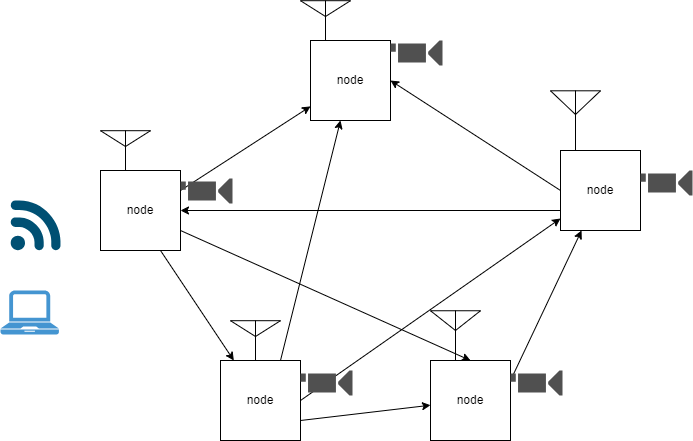
\includegraphics[width=0.5\linewidth]{Images/basic mesh network diagram.png}\par
	    \caption{Basic block diagram of a mesh network}
	
	    \label{Basic block diagram of a mesh network}
	     \end{center}
	\end{figure}

	Each node will be attached to a tree, each having a transceiver